\chapter{Software Architecture}

In this chapter, we will consider the \textbf{general requirements} of a program which will turn accounts into music. At this stage we do not know the specifics of how this will be achieved, therefore the architecture needs to be as versatile as possible.

We will see how we can split the software into two distinct sections. One will handles the input and output operations. the other will do the actual processing to produce music from accounts.

Additionally, the architecture will support a ``plug-in'' framework, allowing many different implementations to be attached with ease.

\begin{figure}[ht]
\centering
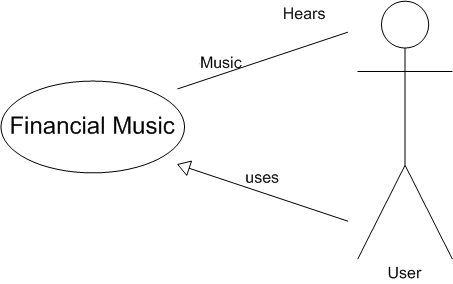
\includegraphics[scale=1.2]{use_case}
\caption{Use case diagram, demonstrating the relationship between the user and the software.}
\label{fig:use_case}
\end{figure}

\section{Requirements of the Framework}

The framework must meet the following requirements:
\begin{enumerate}
\begin{singlespace}
\item Input:
\begin{enumerate}
\item Ability to import accounts from a standard format.
\item Simplicity to add additional methods of importing accounts.
\end{enumerate}
\item Output:
\begin{enumerate}
\item Output in a common music format.
\item Ability to play music.
\end{enumerate}
\item Easy addition of core modules for different methods of generating music from accounts.
\item Versatile framework to allow for high levels of experimentation during development.
\end{singlespace}
\end{enumerate}

\section{The Shell and the Core}

Recall that we mentioned that parts of the software can will fall into two distinct categories. We will term these categories the \textbf{Shell} and the \textbf{Core}. The Shell deals with \textbf{input and output} (I/O) operations such as reading in accounts (input), dealing with file operations (input and output) and playing the music (output).

The Core is where the process of turning accounts into music takes place, and therefore performs the \textbf{processing}.

Looking at the software in this way is essential, as we do not wish to be concerned with issues of input and output (worrying about where the data is coming from or going to) while we are designing processing strategies. Therefore, we should set things up so that the Core doesn't need to be concerned with where the account data is coming from, or what to do with the music that is produced \textit{(figure \ref{fig:shellcore})}.

\begin{figure}[ht]
\centering
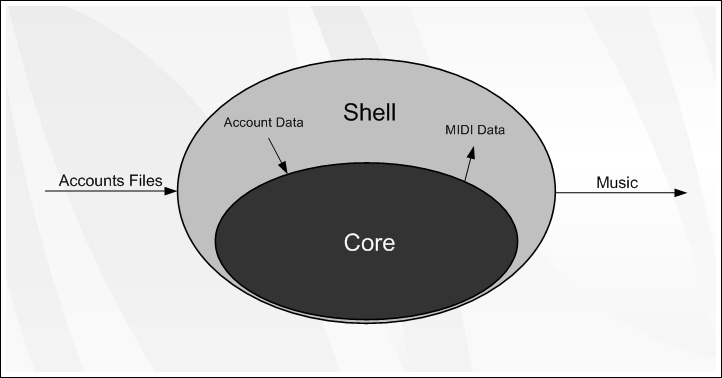
\includegraphics[scale=1.5]{shellcore}
\caption{The relationship between the Shell and the Core in the software's architecture.}
\label{fig:shellcore}
\end{figure}

\section{Languages of Implementation}

Given the differing natures of the Shell and the Core, it is necessary to carefully select a language of implementation that will best suit each task. 

The language chosen for implementation of the Shell is \textbf{Java}. Java is a popular high-level programming language. It also has the advantage of being cross-platform, and web capable.

Java is a suitable language for the tasks the Shell will have to perform, as it has a good selection of class libraries at its disposal for dealing with all the I/O operations that will be required by this project. It has libraries for reading and parsing files. It also has excellent MIDI capabilities.

The Core is concerned purely with mathematical and logical operations which will turn accounts into music, and therefore requires a language which has a syntax oriented towards this end. A functional programming language is a good choice for this, and \textbf{Python} was chosen for this purpose. Python is a high level dynamically typed language, with support for lists, sets and tuples. It supports a functional programming paradigm, inspired by languages such as SML and Haskell. As we will be presenting designs which will be expressed formally, this paradigm will allow focus on the actual processes involved in music generation.

Taking a functional programming approach to writing the core moudules is useful, as it allows us to abstract a problem down to a state where each element of a problem has its own function. This in turn allows the sharing of functions across problems which share many of the same elements.

It also allows functions to be tested individually as they are written. This way, debugging the program is a simpler process; If the integrity of the modules can be verified, then the interactions between modules can be studied in isolation.

(It should be noted however, that the functions developed on the coming pages often display \textit{side-effects} such as displaying text on screen or accessing a global variable, therefore some may not consider the approach truly functional)

As a final point, we need the language used for the core to be able to communicate transparently with the shell. To this end, the core is really implemented in \textbf{Jython}, which is an implementation of the Python language using the \textbf{Java Virtual Machine}.\footnote{The Jython website can be found at: \url{http://www.jython.org}}

\section{Modules of the Shell}

Recall that modules in the shell are responsible mainly for I/O operations, and will be implemented in Java. There are three main classes involved in this:

\begin{itemize}
\begin{singlespace}
\item \texttt{AccountReader.class} -- Reads in the accounts from source files.
\item \texttt{PlayMusic.class} -- Plays music when given a 2 dimensional integer array of MIDI values.
\item \texttt{MusicReader.class} -- Looks for a CSV file with MIDI values and pipes it to \texttt{PlayMusic.class}.
\end{singlespace}
\end{itemize}

\section{Modules of the Core}

Core modules deal with the actual processing. They are as follows:

\begin{itemize}
\begin{singlespace}
\item \texttt{Shared.py} -- Contains functions shared across modules in the Core.
\item \texttt{Settings.py} -- Contains global settings in one location, for easy access.
\item \texttt{Mapping.py} -- Contains function for the Signal Mapping implementation (Chapter 4).
\item \texttt{LSS.py} -- Contains function for the L-System Music Generation implementation (Chapter 5).
\item \texttt{Linden.py} -- Contains functions to implement a generic L-System (also Chapter 5).
\item \texttt{Genome.py} -- Contains functions for the Financial Genome approach (Chapter 7).
\end{singlespace}
\end{itemize}

\section{Module Interactions and Data Flow}

The interactions between modules can be observed in \textit{figure \ref{fig:UML}}.

\begin{figure}[ht]
\centering
\includegraphics[scale=1.5]{UML}
\caption{A UML representation of the interaction between modules in Financial Music.}
\label{fig:UML}
\end{figure}

\section{Platform Requirements}

A system running \textit{Financial Music} will need to meet the following minimum requirements:

\begin{enumerate}
\begin{singlespace}
\item Hardware
\begin{enumerate}
\item MIDI Capabilities
\end{enumerate}
\item Software
\begin{enumerate}
\item Java 1.6.0
\item Jython 2.2.1
\end{enumerate}
\end{singlespace}
\end{enumerate}

\section{Summary}

In this chapter, we have designed and constructed a software architecture to support Financial Music. With a Shell (implemented in Java) and a Core (Implemented in Jython), it will be capable of reading in accounts from an external source, and of playing music using the MIDI standard.

As we develop Python code in the future chapters, we will see an evolution of the Core. However, the Java code of the Shell will remain unchanged, and unaffected by development in the Core.

With a framework in place, we are now ready to begin developing approaches to turning accounts into music, and the next couple of chapters will explore two approaches towards achieving this.